% ===================================================================
%  Week 1 — Session 1: Sampling, Quantization & Color
%  Compile: pdflatex -interaction=nonstopmode slides-a.tex  (twice)
% ===================================================================
\documentclass[10pt,aspectratio=169]{beamer}
% ===================================================================
%  Shared Beamer preamble for "Practical Image Processing"
%  English slides. Compile with pdfLaTeX.
% ===================================================================

\usetheme{metropolis}
\usepackage[T1]{fontenc}
\usepackage[utf8]{inputenc}
\usepackage{lmodern}
\usepackage{listings}
\usepackage{tcolorbox}
\usepackage{fontawesome5}
\usepackage{booktabs}
\usepackage{amsmath,amssymb}
\usepackage{tikz}
\usepackage{pgfplots}
\pgfplotsset{compat=1.17}
\usetikzlibrary{arrows.meta,positioning,shapes.geometric,fit,backgrounds,matrix}
\tcbuselibrary{skins,breakable}

% ---- Palette --------------------------------------------------------
\definecolor{coursePrimary}{HTML}{1B4965}   % deep blue
\definecolor{courseAccent}{HTML}{E76F51}    % coral
\definecolor{courseGood}{HTML}{2A9D8F}      % teal
\definecolor{courseBad}{HTML}{C0392B}       % red
\definecolor{courseInfo}{HTML}{2980B9}      % blue
\definecolor{codeBg}{HTML}{F5F6FA}
\definecolor{codeKw}{HTML}{8E44AD}
\definecolor{codeStr}{HTML}{2A9D8F}
\definecolor{codeCom}{HTML}{7F8C8D}

\setbeamercolor{frametitle}{bg=coursePrimary}
\setbeamercolor{progress bar}{fg=courseAccent}
\setbeamercolor{alerted text}{fg=courseAccent}
\metroset{block=fill,sectionpage=progressbar,numbering=fraction}

% ---- Code listings (Python is built into listings) -----------------
\lstdefinestyle{course}{
  backgroundcolor=\color{codeBg},
  basicstyle=\ttfamily\scriptsize,
  keywordstyle=\color{codeKw}\bfseries,
  stringstyle=\color{codeStr},
  commentstyle=\color{codeCom}\itshape,
  numberstyle=\tiny\color{codeCom},
  numbers=left, numbersep=6pt,
  showstringspaces=false, breaklines=true, breakatwhitespace=true,
  tabsize=4, columns=fullflexible,
  frame=single, framesep=4pt, rulecolor=\color{gray!30},
  keepspaces=true, upquote=true, language=Python,
}
\lstset{style=course}
\lstdefinelanguage{bash}{
  keywords={cd,pip,python,venv,source,import}, sensitive=true,
  morecomment=[l]{\#}, morestring=[b]', morestring=[b]",
}

% ---- Reusable callout boxes ----------------------------------------
\newtcolorbox{goodbox}[1][Good practice]{colback=courseGood!8,colframe=courseGood,
  fonttitle=\bfseries,title={\faCheck~#1},boxrule=0.6pt,left=4pt,right=4pt,top=3pt,bottom=3pt}
\newtcolorbox{badbox}[1][Pitfall]{colback=courseBad!8,colframe=courseBad,
  fonttitle=\bfseries,title={\faTimes~#1},boxrule=0.6pt,left=4pt,right=4pt,top=3pt,bottom=3pt}
\newtcolorbox{infobox}[1][Note]{colback=courseInfo!8,colframe=courseInfo,
  fonttitle=\bfseries,title={\faInfoCircle~#1},boxrule=0.6pt,left=4pt,right=4pt,top=3pt,bottom=3pt}
\newtcolorbox{mathbox}[1][Math]{colback=coursePrimary!6,colframe=coursePrimary,
  fonttitle=\bfseries,title={\faCalculator~#1},boxrule=0.6pt,left=4pt,right=4pt,top=3pt,bottom=3pt}

\newcommand{\keyidea}[1]{\begin{alertblock}{Key idea}#1\end{alertblock}}
\newcommand{\term}[1]{\textbf{\color{coursePrimary}#1}}
\newcommand{\code}[1]{\lstinline[basicstyle=\ttfamily\small]|#1|}

% ---- A helper to draw a small pixel grid, cells shaded by value ----
% \pixelgrid{ {10,20,120,200,240}, {30,60,130,180,230}, ... }
\newcommand{\pixelgrid}[1]{%
  \begin{tikzpicture}[font=\scriptsize,scale=0.6]
    \foreach \row [count=\ry] in {#1} {
      \foreach \val [count=\cx] in \row {
        \draw[gray,fill=coursePrimary!8] (\cx,-\ry) rectangle ++(1,-1);
        \node at (\cx+0.5,-\ry-0.5) {\val};
      }
    }
  \end{tikzpicture}}


\title{Digital Images \& the Pipeline}
\subtitle{Week 1 — Session 1: Sampling, Quantization \& Color}
\author{Practical Image Processing}
\date{Lecture 1.1 \textbullet\ 60--70 min}

\begin{document}

\maketitle

\begin{frame}{Where this course is going}
  \begin{columns}[T]
    \begin{column}{0.56\textwidth}
      By the end you will build \alert{DocScan}: a photo of a document $\rightarrow$ a clean,
      deskewed, machine-readable scan, then read it with a small neural net.
      \begin{itemize}
        \item Tools: \term{Python + OpenCV + NumPy}.
        \item Weeks 1--11: classical image processing.
        \item Weeks 12--14: an introduction to deep learning for vision.
      \end{itemize}
    \end{column}
    \begin{column}{0.44\textwidth}
      \begin{alertblock}{The habit we build}
        Understand the pixels and the math \emph{first}; call the library second; reach for a
        neural net only when classical methods run out.
      \end{alertblock}
    \end{column}
  \end{columns}
\end{frame}

\begin{frame}{The image-processing pipeline}
  \begin{center}
  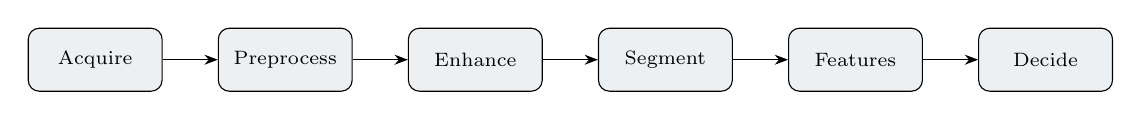
\begin{tikzpicture}[font=\scriptsize,>=Stealth,node distance=3mm and 7mm,
    b/.style={draw,rounded corners,fill=coursePrimary!8,minimum height=8mm,minimum width=17mm,align=center}]
    \node[b] (acq){Acquire};
    \node[b,right=of acq] (pre){Preprocess};
    \node[b,right=of pre] (enh){Enhance};
    \node[b,right=of enh] (seg){Segment};
    \node[b,right=of seg] (feat){Features};
    \node[b,right=of feat] (dec){Decide};
    \draw[->](acq)--(pre);\draw[->](pre)--(enh);\draw[->](enh)--(seg);\draw[->](seg)--(feat);\draw[->](feat)--(dec);
  \end{tikzpicture}
  \end{center}
  \keyidea{Every task in this course is some path through this pipeline. DocScan walks all of it.}
\end{frame}

\begin{frame}{Two sessions this week}
  \begin{columns}[T]
    \begin{column}{0.5\textwidth}
      \begin{infobox}[Today — Session 1]
        What an image \emph{is}. Sampling, quantization, resolution, bit depth, and color.
        The vocabulary and the numbers behind every pixel.
      \end{infobox}
    \end{column}
    \begin{column}{0.5\textwidth}
      \begin{infobox}[Next — Session 2]
        Images \emph{in code}. NumPy arrays, formats, and the physical imaging model
        (noise, aliasing, gamma). Ends with the week's deliverable.
      \end{infobox}
    \end{column}
  \end{columns}
  \vspace{4pt}
  Same running examples throughout: a \term{water-meter} numerator and a license
  \term{plate} crop from our real dataset.
\end{frame}

\begin{frame}{Roadmap}\tableofcontents\end{frame}

% ==================================================================
\section{What is a digital image?}
% ==================================================================

\begin{frame}{An image is a function, sampled onto a grid}
  \begin{itemize}
    \item A continuous image is a function $f(x,y)$ = brightness at position $(x,y)$.
    \item A \term{digital} image samples it on a grid and rounds each value: \term{pixels}.
    \item A grayscale image is a 2D array; a color image is 3 such arrays (channels).
  \end{itemize}
  \begin{mathbox}
    $f(x,y)$, with $x=0\dots W{-}1$, $y=0\dots H{-}1$, and each value in $\{0,\dots,255\}$ (8-bit).
  \end{mathbox}
\end{frame}

\begin{frame}{From continuous scene to discrete array}
  \begin{center}
  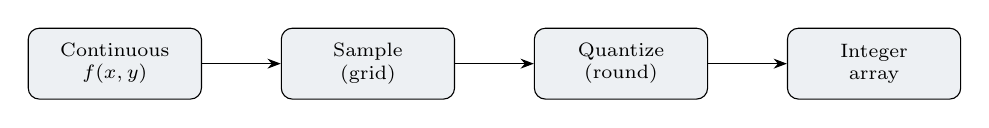
\begin{tikzpicture}[font=\scriptsize,>=Stealth,node distance=4mm and 10mm,
    b/.style={draw,rounded corners,fill=coursePrimary!8,minimum height=9mm,minimum width=22mm,align=center}]
    \node[b] (cont){Continuous\\$f(x,y)$};
    \node[b,right=of cont] (samp){Sample\\(grid)};
    \node[b,right=of samp] (quant){Quantize\\(round)};
    \node[b,right=of quant] (arr){Integer\\array};
    \draw[->](cont)--(samp);\draw[->](samp)--(quant);\draw[->](quant)--(arr);
  \end{tikzpicture}
  \end{center}
  \begin{itemize}
    \item \term{Sampling} chops space into a grid: \emph{where} we measure.
    \item \term{Quantization} rounds each brightness to a level: \emph{how precisely} we record it.
    \item Two knobs, two kinds of loss — the whole of this section.
  \end{itemize}
\end{frame}

\begin{frame}{Pixels are just numbers}
  \begin{columns}[T]
    \begin{column}{0.5\textwidth}
      A tiny 5$\times$5 patch of intensities:
      \begin{center}
      \pixelgrid{
        {10,20,120,200,240},
        {30,60,130,180,230},
        {50,90,150,190,220},
        {70,110,160,200,250},
        {90,130,170,210,255}
      }
      \end{center}
    \end{column}
    \begin{column}{0.5\textwidth}
      \begin{itemize}
        \item 0 = black, 255 = white, values between = gray.
        \item ``Processing'' an image = doing arithmetic on these numbers.
        \item There is no magic: every operation is math on an array.
      \end{itemize}
    \end{column}
  \end{columns}
\end{frame}

\begin{frame}{Reading the grid: indexing a pixel}
  \begin{columns}[T]
    \begin{column}{0.52\textwidth}
      Same 5$\times$5 patch, now with indices. In image code we write \code{img[row, col]}:
      \begin{itemize}
        \item \code{img[0,0]} = 10 (top-left).
        \item \code{img[2,3]} = 190 (row 2, column 3).
        \item \code{img[4,4]} = 255 (bottom-right, pure white).
      \end{itemize}
    \end{column}
    \begin{column}{0.48\textwidth}
      \begin{center}
      \pixelgrid{
        {10,20,120,200,240},
        {30,60,130,180,230},
        {50,90,150,190,220},
        {70,110,160,200,250},
        {90,130,170,210,255}
      }
      \end{center}
    \end{column}
  \end{columns}
  \begin{infobox}
    Row first, then column. This is $[y,x]$, the \emph{reverse} of math's $(x,y)$ — more on that in Session 2.
  \end{infobox}
\end{frame}

\begin{frame}{A real image from our dataset}
  \begin{columns}[T]
    \begin{column}{0.5\textwidth}
      \begin{center}
      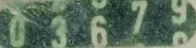
\includegraphics[width=\linewidth]{../assets/meter_bgr.png}\\[2pt]
      {\scriptsize original (color) — a water-meter numerator}
      \end{center}
    \end{column}
    \begin{column}{0.5\textwidth}
      \begin{center}
      
\includegraphics[width=\linewidth]{../assets/meter_gray.png}\\[2pt]
      {\scriptsize grayscale — one channel, same structure}
      \end{center}
    \end{column}
  \end{columns}
  \vspace{4pt}
  This 48$\times$196 crop is our running example. Reading these digits is exactly what the
  DocScan capstone builds toward. (Data: \code{E:/data/abfa\_image/numerators}.)
\end{frame}

\begin{frame}{Sampling: how finely we measure space}
  \begin{center}
  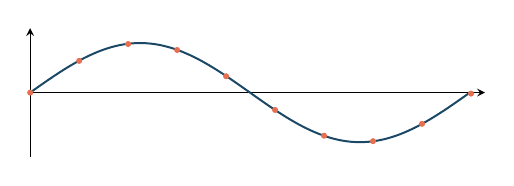
\begin{tikzpicture}[scale=0.9]
    \begin{axis}[width=8cm,height=3.4cm,ticks=none,axis lines=middle,
      xmin=0,xmax=6.5,ymin=-1.3,ymax=1.3,clip=false,font=\tiny]
      \addplot[coursePrimary,thick,domain=0:6.3,samples=100]{sin(deg(x))};
      \addplot[courseAccent,only marks,mark=*,mark size=1pt]
        coordinates{(0,0)(0.7,0.64)(1.4,0.98)(2.1,0.86)(2.8,0.33)(3.5,-0.35)(4.2,-0.87)(4.9,-0.98)(5.6,-0.63)(6.3,-0.02)};
    \end{axis}
  \end{tikzpicture}
  \end{center}
  \term{Sampling} = choosing grid points (resolution). Too few samples and detail is lost —
  or worse, faked (aliasing, Session 2). More pixels = more spatial detail, more data.
\end{frame}

\begin{frame}{Sampling, made concrete}
  Our meter crop is $196$ wide $\times\,48$ tall. That is our sampling grid.
  \begin{mathbox}[Worked example]
    A digit stroke about \(1.5\) px wide is barely resolved. Halve the width to $98\times24$
    and the stroke spans $<1$ px — the digit becomes unreadable. \\[3pt]
    Total samples: \(196 \times 48 = 9{,}408\) pixels. Halving each side: \(98\times24 = 2{,}352\)
    — one quarter the samples.
  \end{mathbox}
  \begin{itemize}
    \item Halving \emph{each} linear dimension quarters the pixel count (area scales as the square).
    \item So ``a bit more resolution'' costs a lot more data — budget it deliberately.
  \end{itemize}
\end{frame}

\begin{frame}{Quantization: how finely we measure brightness}
  \begin{itemize}
    \item \term{Quantization} = rounding each sample to a finite set of levels (the bit depth).
    \item 8-bit = 256 levels (0--255); 1-bit = black/white; 16-bit = 65{,}536 (medical/RAW).
    \item Too few levels $\rightarrow$ visible \term{banding} in smooth gradients.
  \end{itemize}
  \begin{infobox}
    Resolution (sampling) and bit depth (quantization) are the two axes of ``how much image.''
  \end{infobox}
\end{frame}

\begin{frame}{Quantization, made concrete}
  \begin{mathbox}[Worked example]
    An intensity of \(162\) stored at different bit depths, level size \(= 256/2^{b}\): \\[3pt]
    \begin{tabular}{@{}llll@{}}
      \toprule
      bits \(b\) & levels \(2^b\) & step & \(162\) snaps to \\
      \midrule
      8 & 256 & 1   & 162 \\
      4 & 16  & 16  & 160 \\
      2 & 4   & 64  & 192 \\
      1 & 2   & 128 & 255 \\
      \bottomrule
    \end{tabular}
  \end{mathbox}
  \begin{itemize}
    \item Fewer bits = coarser steps = bigger rounding error, then visible banding.
    \item 8-bit's step of 1 is below what the eye resolves on a normal display — hence the standard.
  \end{itemize}
\end{frame}

\begin{frame}{Resolution, size, and memory}
  \begin{itemize}
    \item A $W\times H$ grayscale 8-bit image is $W\cdot H$ bytes; color is $3\times$ that.
    \item A 12-megapixel color photo $\approx$ 36\,MB \emph{uncompressed}.
    \item That's why formats compress — and why processing big images needs care (Week 11).
  \end{itemize}
  \begin{mathbox}[Worked example]
    A $4000\times3000$ color photo: \(4000 \times 3000 = 12{,}000{,}000\) px.
    Grayscale: \(12\) MB. Color (3 bytes/px): \(36\) MB. Our meter crop: \(9{,}408 \times 3 \approx 28\) KB.
  \end{mathbox}
  \keyidea{Know your image's shape and dtype before anything else: \code{img.shape}, \code{img.dtype}.}
\end{frame}

% ==================================================================
\section{Color}
% ==================================================================

\begin{frame}{Color: three numbers per pixel}
  \begin{itemize}
    \item \term{RGB}: red, green, blue channels; how screens emit light.
    \item A color pixel is a triple $(R,G,B)$, each 0--255.
    \item Grayscale collapses color to one intensity — often the first step (less data, same structure).
  \end{itemize}
  \begin{mathbox}
    Luminance: $Y = 0.299R + 0.587G + 0.114B$ — green dominates because our eyes do.
  \end{mathbox}
\end{frame}

\begin{frame}{Luminance vs the naive average}
  \begin{mathbox}[Worked example]
    Take a pixel \((R,G,B) = (120,\,200,\,80)\). \\[3pt]
    Perceptual luminance:
    \(Y = 0.299(120) + 0.587(200) + 0.114(80) = 35.9 + 117.4 + 9.1 = 162.4 \approx 162.\) \\[3pt]
    Naive average:
    \((120 + 200 + 80)/3 = 400/3 = 133.3 \approx 133.\)
  \end{mathbox}
  \begin{itemize}
    \item The two differ by \(\approx 29\) levels — the green-heavy pixel looks \emph{brighter}
      than the flat average admits.
    \item Averaging under-weights green and over-weights blue relative to human vision.
  \end{itemize}
\end{frame}

\begin{frame}{Why convert to grayscale}
  \begin{itemize}
    \item Many operations (edges, thresholds) need intensity, not color — 1 channel, 3$\times$ less work.
    \item DocScan works mostly in grayscale; color returns only when it carries information.
    \item But grayscale \emph{discards} information — don't do it if hue matters (Week 8 color segmentation).
  \end{itemize}
  \begin{badbox}
    Averaging $(R+G+B)/3$ is a common shortcut — but the weighted luminance is perceptually correct.
  \end{badbox}
\end{frame}

\begin{frame}{Other color spaces, and why}
  \begin{center}
  \begin{tabular}{@{}lll@{}}
    \toprule
    \textbf{Space} & \textbf{Channels} & \textbf{Good for} \\
    \midrule
    RGB & red, green, blue & storage, display \\
    Grayscale & intensity & most classical processing \\
    HSV & hue, saturation, value & color-based selection (robust to lighting) \\
    Lab & lightness, a, b & perceptual distance, color correction \\
    \bottomrule
  \end{tabular}
  \end{center}
  \keyidea{Choosing the right color space can make a hard problem easy — e.g. ``find the red object'' is trivial in HSV, painful in RGB.}
\end{frame}

\begin{frame}{HSV intuition}
  \begin{itemize}
    \item \term{Hue}: which color (angle on the color wheel). \term{Saturation}: how vivid. \term{Value}: how bright.
    \item Separating color from brightness makes selection robust to shadows and lighting.
    \item ``All the red pixels'' = a hue range — one threshold, done.
  \end{itemize}
  \begin{infobox}
    Hue is an angle $0$--$360^\circ$ (OpenCV halves it to fit $0$--$179$ in a byte). Red sits near both ends.
  \end{infobox}
\end{frame}

\begin{frame}{Value is (almost) grayscale}
  \begin{columns}[T]
    \begin{column}{0.5\textwidth}
      \begin{center}
      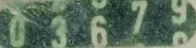
\includegraphics[width=\linewidth]{../assets/meter_bgr.png}\\[2pt]
      {\scriptsize color meter crop (BGR)}
      \end{center}
    \end{column}
    \begin{column}{0.5\textwidth}
      \begin{center}
      
\includegraphics[width=\linewidth]{../assets/meter_value.png}\\[2pt]
      {\scriptsize the V (value) channel of HSV}
      \end{center}
    \end{column}
  \end{columns}
  \vspace{3pt}
  \begin{itemize}
    \item \code{V = max(R,G,B)} — the brightest channel per pixel, so it tracks intensity.
    \item Close to grayscale but not identical: luminance weights channels; value just takes the max.
  \end{itemize}
\end{frame}

\begin{frame}{Color helps: picking out the plate}
  \begin{columns}[T]
    \begin{column}{0.5\textwidth}
      \begin{center}
      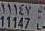
\includegraphics[width=\linewidth]{../assets/plate_bgr.png}\\[2pt]
      {\scriptsize a license-plate crop, in color}
      \end{center}
    \end{column}
    \begin{column}{0.5\textwidth}
      \begin{center}
      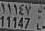
\includegraphics[width=\linewidth]{../assets/plate_gray.png}\\[2pt]
      {\scriptsize grayscale — hue is gone}
      \end{center}
    \end{column}
  \end{columns}
  \vspace{3pt}
  \begin{itemize}
    \item If the task were ``find the colored region,'' HSV would isolate it by hue in one step.
    \item Once located, the \emph{reading} of the characters happens in grayscale — best of both.
  \end{itemize}
\end{frame}

% ==================================================================
\section{In-class exercise}
% ==================================================================

\begin{frame}{\faPen~In-class exercise (10 min)}
  \begin{infobox}[Predict, then compute by hand]
    Work in your notebook first; check with code only after you have an answer.
  \end{infobox}
  A single pixel has \((R,G,B) = (60,\,180,\,90)\).
  \begin{enumerate}
    \item Compute its \term{luminance} \(Y = 0.299R + 0.587G + 0.114B\).
    \item Compute the \term{naive average} \((R+G+B)/3\). How far apart are they?
    \item An $800\times600$ color image: how many bytes uncompressed? In grayscale?
    \item At 2-bit depth (4 levels, step 64), what does the value \(90\) round to?
  \end{enumerate}
\end{frame}

\begin{frame}{\faPen~Debrief}
  \begin{itemize}
    \item \(Y = 0.299(60) + 0.587(180) + 0.114(90) = 17.9 + 105.7 + 10.3 = 133.9 \approx 134.\)
    \item Average \(= (60+180+90)/3 = 330/3 = 110.\) They differ by \(\approx 24\) — green pulls \(Y\) up.
    \item \(800\times600 = 480{,}000\) px \(\Rightarrow 1.44\) MB color, \(480\) KB grayscale.
    \item Step 64: \(90\) lands between \(64\) and \(128\); nearest level is \(64\) (since \(90-64=26 < 128-90=38\)).
  \end{itemize}
  \keyidea{Every ``processing'' step you'll ever write is arithmetic like this, done to millions of pixels at once.}
\end{frame}

\begin{frame}{Common pitfalls this session}
  \begin{columns}[T]
    \begin{column}{0.5\textwidth}
      \begin{badbox}
        Down-sizing too far destroys thin strokes — a $196\times48$ digit crop halved is unreadable.
      \end{badbox}
      \begin{badbox}[Wrong gray]
        \((R+G+B)/3\) is not perceptual gray; use the luminance weights.
      \end{badbox}
    \end{column}
    \begin{column}{0.5\textwidth}
      \begin{goodbox}
        Always know \code{shape} and \code{dtype} before you touch a pixel.
      \end{goodbox}
      \begin{goodbox}[Right tool]
        Pick the color space for the task: HSV to \emph{find} color, grayscale to \emph{read} structure.
      \end{goodbox}
    \end{column}
  \end{columns}
\end{frame}

\begin{frame}{What you should now be able to do}
  \begin{itemize}
    \item Explain sampling and quantization, and the loss each one introduces.
    \item Relate resolution and bit depth to file size and memory with a quick calculation.
    \item Convert a color pixel to luminance by hand, and say why it beats the average.
    \item Choose between RGB, grayscale, and HSV for a given goal.
  \end{itemize}
  \keyidea{An image is a function sampled onto a grid and rounded — two knobs, two kinds of loss.}
\end{frame}

\begin{frame}[standout]
  Next session
  \vspace{4pt}
  \normalsize These numbers live inside a \term{NumPy array}. Session 2 loads real images in code,
  meets the \code{uint8} overflow trap, picks file formats, and traces where pixels physically
  come from — then sets the week's deliverable.
\end{frame}

\end{document}
